\normaltrue \difficilefalse \tdifficilefalse
\correctiontrue

%\UPSTIidClasse{11} % 11 sup, 12 spé
%\newcommand{\UPSTIidClasse}{12}

\exer{Système vis-écrou $\star$ \label{TEC:04:Jeq:36}}
\marginnote{\textit{D'après ressources Pole Chateaubriand -- Joliot-Curie.}}
\setcounter{question}{0}\
\marginnote{\xpComp{TEC}{04}}
\ifcorrection
\else
\marginnote{\textbf{Pas de corrigé pour cet exercice.}}
\fi

\ifprof
\else
Soit la chaîne de transmission suivante. 
\begin{marginfigure}
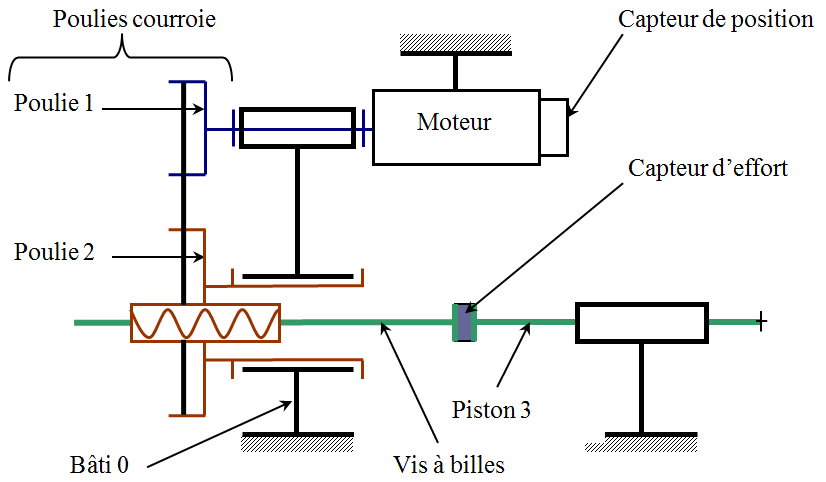
\includegraphics[width=\linewidth]{36_01}
\end{marginfigure}

Le schéma du restituteur actif est donné ci-dessous. Le pas de la vis est $p_v =\SI{10}{mm}$.
Le diamètre de la poulie 2 est le double de celui de la poulie 1. 

\fi


%\question{Sur le schéma cinématique, repasser chaque solide d’une couleur différente.}
%\ifprof
%\else
%\fi

\question{Réaliser la chaîne d’énergie-puissance partielle en définissant les noms des transmetteurs et les grandeurs
d’entrée et de sortie cinématiques.}
\ifprof ~\\
\else
\fi

\question{Définir la loi entrée-sortie entre la vitesse de translation du piston 3 et la vitesse de rotation du moteur~1. }
\ifprof~\\
%On a $Z_3 = 2Z_2 + Z_1$.
\else
\fi

On note $J_i$ le moment d'inertie de la pièce $i$ autour de son axe de rotation. On note $M$ la masse de l'ensemble piston 3 -- Vis à billes -- Capteur d'effort. 
\question{ Déterminer le moment d'inertie équivalent ramené à l'arbre moteur.}
\ifprof ~\\
\else
\fi

\question{Déterminer la masse équivalente ramenée au mouvement du piston.}
\ifprof ~\\
\else
\fi


\ifprof
\else

\marginnote{Corrigé voir \ref{TEC:04:Jeq:36}.}

\fi